\documentclass[11pt]{article}
%\usepackage{enumerate}
%\usepackage{fullpage}
\usepackage{graphicx}
\usepackage{amssymb}
\usepackage{amsmath}
\usepackage{subcaption}
\usepackage{bm}
\usepackage{float}
\usepackage{fancyhdr}
\usepackage{listings}
\usepackage{color}
\usepackage{hyperref}



\pagestyle{fancy}
\fancyhead{}
\fancyhead[L]{Epidemic Modeller Project Overview — Alex Gardner}
\fancyfoot{}
\fancyfoot[C]{\thepage}

\setlength{\headheight}{14pt}

\begin{document}
\title{Epidemic Modeller Project Overview}
\author{Alex Gardner}
\date{MA4J5}
\maketitle

\section*{Introduction}
In this project, I've tried to create a stochastic spatial method of simulating epidemics. I hope that when using completely random movement we get simulations very similar to existing basic methods (like a simple Gillespie stochastic SEIR model), but we could modify this new spatial model to include patterns of movement and then compare the effects of different movement patterns to find new insights.

Another aim of this project is to provide a visual representation of an epidemic. Just looking at graphs of infection levels wouldn't help a school student or member of the public gain intuition on the exponential nature of disease spread, but a model that can be visualised can be used to teach a broader audience on how a new disease spreads through a population, and the effects that interventions have.

Though while the models I create here are overly simplistic, and the renderers I create are not very visually appealing, they could be improved upon and then used to educate larger numbers of people on epidemiology and the importance of the interventions that governments impose. This method makes understanding epidemiology accessible to people who are less educated and, when taught to the wider public, could help inspire public trust in governments implementing strict measures.

The models I create in this project are likely too simple to apply to humans, and wouldn't provide much benefit over a standard Gillespie stochastic SEIR model, but might more closely resemble a different species' nest or colony. Modifying the movement of the individuals to be like bees, bats or ants should not be a difficult extension of the models presented below.

\section*{Basic Visual Model}
In this model, we create a model which is stochastic, and where the individuals in the population move in straight lines in random directions. Each individual will be in either the susceptible class, the exposed class, the infectious class, or the removed class at any one time. We choose to move individuals between classes according to realisations of gamma distributions, except for when an infectious individual infects others around them — where we use the exponential distribution. Gamma distributions are great for this use case as often people tend to be infected a random duration of time, say between $n$ and $k$ days, and gamma random variables can encapsulate this property and they tend to have a large mass near the mean of the distribution. They are also sums of exponential random variables, a property that we exploit to make feasible the mathematical analysis of the model I set up.

\subsection*{Setup}
We start with a region $A=[0,1]\times [0,1]$, and each individual $i$ has coordinates $(x_i, y_i)\in A$. Each individual starts with coordinates $x_i \sim U[0,1]$, $y_i \sim U[0,1]$, and has velocity $\frac{dx_i(t)}{dt} \sim U[-v,v]$, $\frac{dy_i(t)}{dt} \sim U[-v,v]$ for some speed parameter $v$. Whenever an individual hits the boundary, e.g. $x_i=0$, then they 'bounce' off of the boundary by negating the velocity in the $x$ or $y$ component, whichever boundary we hit.

\begin{figure}[H]
\label{BasicModelDiagram}
\begin{center}
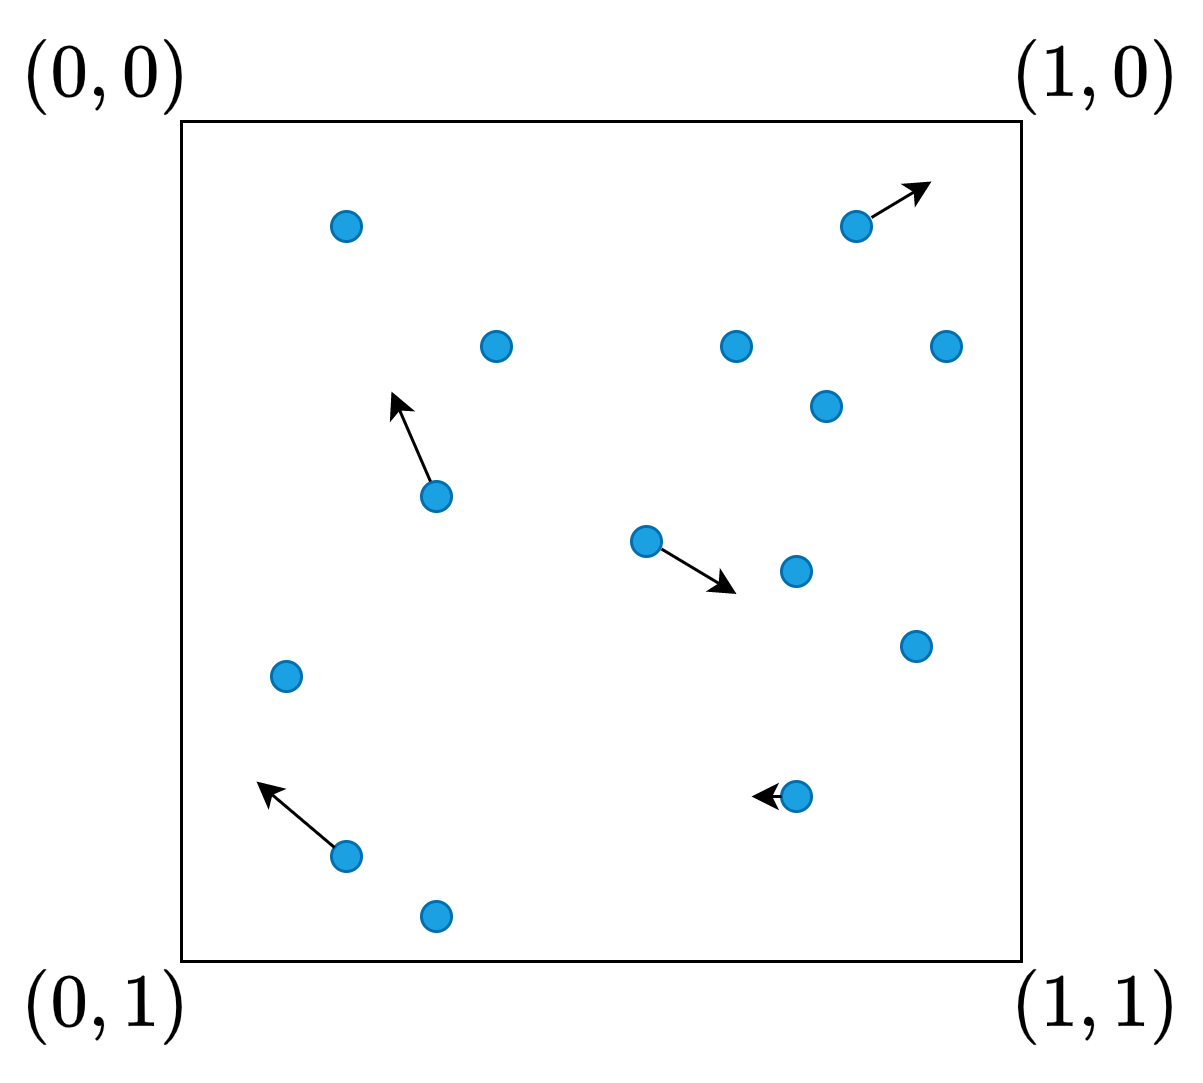
\includegraphics[width=0.6\textwidth]{BasicModelDiagram1}
\end{center}
\end{figure}

Each individual has state $s_i\in \{S,E,I,R\}$ and our model starts with $N_S$ people in the S class, $N_I$ in the I class, $N_E$ in the E class, and $N_R$ in the R class. When an individual enters the E class (after getting infected, or by initial condition), then they get assigned a time when their latency period will end, which is distributed $t_L \sim \text{Gamma}(\sigma)$. When an individual enters the I class, they get assigned a time when their infection period will end, which is distributed $t_R \sim \text{Gamma}(\frac{1}{\gamma\lambda}, \lambda)$. Also when an individual enters the I class, they get assigned a time at which they will next attempt to infect, with distribution $t_I\sim \text{Exp}(\lambda)$. Once an infectious person attempts to infect, they get assigned the next time when they will infect (with the same distribution), though they won't be able to attempt to infect any more if they recover before the time to next infect attempt.

We also discretise time and have it increment by a fixed amount each step in a while loop (I've used 0.1 days time-step as the default), and in each iteration we calculate the new locations of the individuals and check if any events occurred since the previous time-step, and then apply the effects of the events that have happened and schedule new events in the future (e.g. if an event causes a new individual to join the exposed class, randomly generate the length of time they will stay in the $E$ class and schedule the end-of-latency-period event to happen at the time in the future).
\subsubsection*{Infect attempts}
Whenever an individual attempts to infect, we check if there is at least one other individual within $l^1$ distance $\frac{b}{\sqrt{N}}$. We choose this distance because there is $1/N$ area per individual in the region $A$, and if that were a square it would have side length $1/\sqrt{N}$, and then we just multiply that by a scalar parameter $b$ which we can choose when setting up the model. If there is no susceptible people in the area then the attempt failed and nobody new got infected. If there was at least one susceptible individual nearby, then one of them gets picked and enters the exposed class.

\subsection*{Analysis}
The recovery rate $\gamma$ is the inverse of the average number of days spent in the I class. Hence why time spent in the infectious class $t_R \sim \text{Gamma}(\frac{1}{\gamma\lambda}, \lambda)$ was chosen, because $\mathbb{E}(t_R)=\frac{1}{\gamma\lambda} \lambda=\frac{1}{\gamma}$.

The number of people in an $l^1$ radius $\frac{b}{\sqrt{N}}$ of an infectious individual's position would be effectively distributed with $m\sim \text{Binomial}(S,b/N)$. Hence the probability that there is at least 1 susceptible individual in that area will be $\mathbb{P}(m\geq 1) = 1-\mathbb{P}(m=0) = 1-(1-\frac{b}{N})^S$. This gives us the probability that a given infection attempt will be successful.

Approximating $R_0$: First we assume that $S\approx N$ for calculating the average number of people that the first person will infect. This allows us to simplify our above probability for a successful infection attempt $1-(1-\frac{b}{N})^S\approx 1-\exp(-b)$. For the first infectious individual, the time taken between each infection attempt is distributed $t_I\sim \text{Exp}(\lambda)$ and the time taken to recovery is $t_R \sim \text{Gamma}(\frac{1}{\gamma\lambda}, \lambda)$. This was chosen so that the average length of infection was $1/\gamma$ and because $\text{Gamma}(\frac{1}{\gamma\lambda}, \lambda)$ is effectively the sum of $\frac{1}{\gamma\lambda}$ of $\text{Exp}(\lambda)$ random variables, so the average number of infection attempts over the duration of the first infection should be $\frac{1}{\gamma\lambda}$. This means that $R_0\approx\frac{1}{\gamma\lambda}(1-\exp(-b))$. And so our contact rate $\beta$ should be approximately $\frac{1}{\lambda}(1-\exp(-b))$.

So, with this result, given a $\beta$ value, we can fix either $\lambda$ or $b$ and then calculate the value of the other parameter that we didn't fix so that $\beta = \frac{1}{\lambda}(1-\exp(-b))$.

\subsection*{Implementation}
I implement the model in Python and create a renderer to display what's going on in the model throughout the simulated outbreak.
%TODO explain code structure

\subsection*{Simulation results and renders}

%TODO add videos of example run throughs.

\section*{Compartment Model}
This model is very similar to the Basic Model defined above, but with this model we have multiple of the previous model running side by side, each called compartments, and individuals occasionally move between the different compartments — which could represent different towns/villages in a region.
\subsection*{Setup}
As this is an extension of the previous model, we use the setup defined previously, and create $n$ different compartments. Each compartment starts with its own set of initial conditions. We will usually start with only one of the compartments having a single infected individual, with the rest of the compartments having none.

For travellers between compartments, we introduce a mixing rate $m$, defined as the probability that anyone in a single compartment leaves to travel towards a different compartment. They then spend some fixed time $t_{\text{travel}}$ (some number of days) travelling to a randomly selected compartment (other than from the one they are starting at). During transit, infectious individuals can't infect anyone else and susceptibles can't get infected while in transit (this doesn't happen in the real world when using public transport, though I've just done it for the sake of model simplicity). After a traveller arrives in a compartment they become another individual in that compartment and start moving around it in a random direction. They don't return to their original compartment, which is another issue with the model that I should have planned when designing it originally. I didn't go back and fix this as I've already spent a while on this project and the current solution is good enough to demonstrate the behaviour of different communities getting infected at different times during the outbreak.

\subsection*{Implementation}
%TODO implementation

\subsection*{Simulation results and renders}

%TODO add videos of example run throughs.

\section*{Closing Remarks}

\end{document}
